\chapter*{附\qquad 录}

\section*{附录~1\quad	课程管理系统业务过程模型}
\label{sec:appendix-bpm}

本节为图~\ref{BPMOverview} 提供展开补充。

\begin{figure}[!hbp]
  \begin{center}
    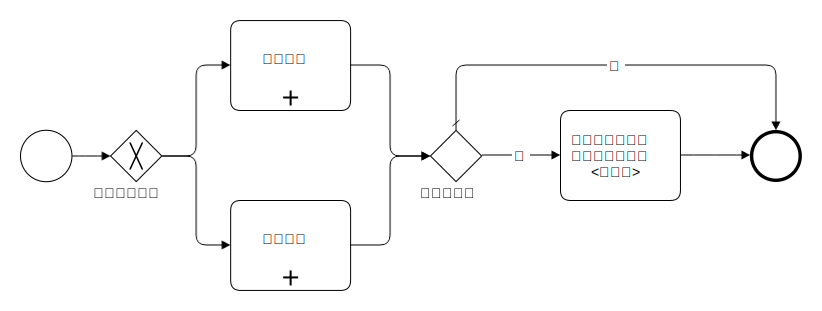
\includegraphics[width=\textwidth]{figures/bpm-cs.pdf}
    业务过程模型示意图(选课)\label{BPMCourseRegister}
  \end{center}
\end{figure}

\begin{figure}[!hbp]
  \begin{center}
    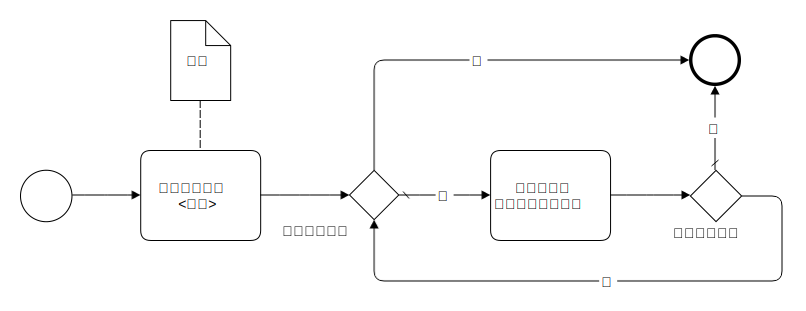
\includegraphics[width=\textwidth]{figures/bpm-cs-pref.pdf}
    业务过程模型示意图(选课-志愿)\label{BPMCourseRegisterP}
  \end{center}
\end{figure}

\begin{figure}[!hbp]
  \begin{center}
    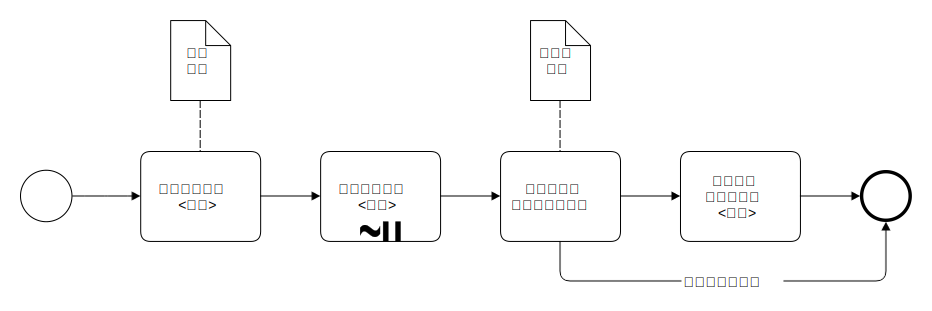
\includegraphics[width=\textwidth]{figures/bpm-cs-dual.pdf}
    业务过程模型示意图(选课-双选)\label{BPMCourseRegisterD}
  \end{center}
\end{figure}

\begin{figure}[!hbp]
  \begin{center}
    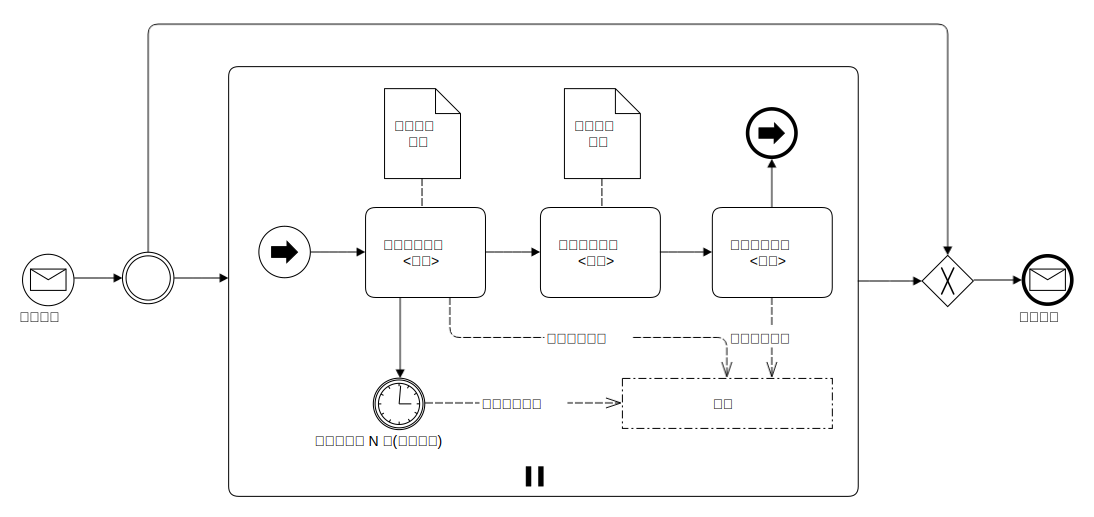
\includegraphics[width=\textwidth]{figures/bpm-task.pdf}
    业务过程模型示意图(课程任务)\label{BPMTask}
  \end{center}
\end{figure}

\newpage

\section*{附录~2\quad	课程管理系统产品需求表格}
\label{sec:appendix-requirement-table}

\LTXtable{\linewidth}{parts/table/requirement.tex}

\newpage

\section*{附录~3\quad	数据库设计示意图}
\label{sec:appendix-database-diagram}

下图展示完整的数据库设计视图:

\begin{figure}[!h]
  \begin{center}
    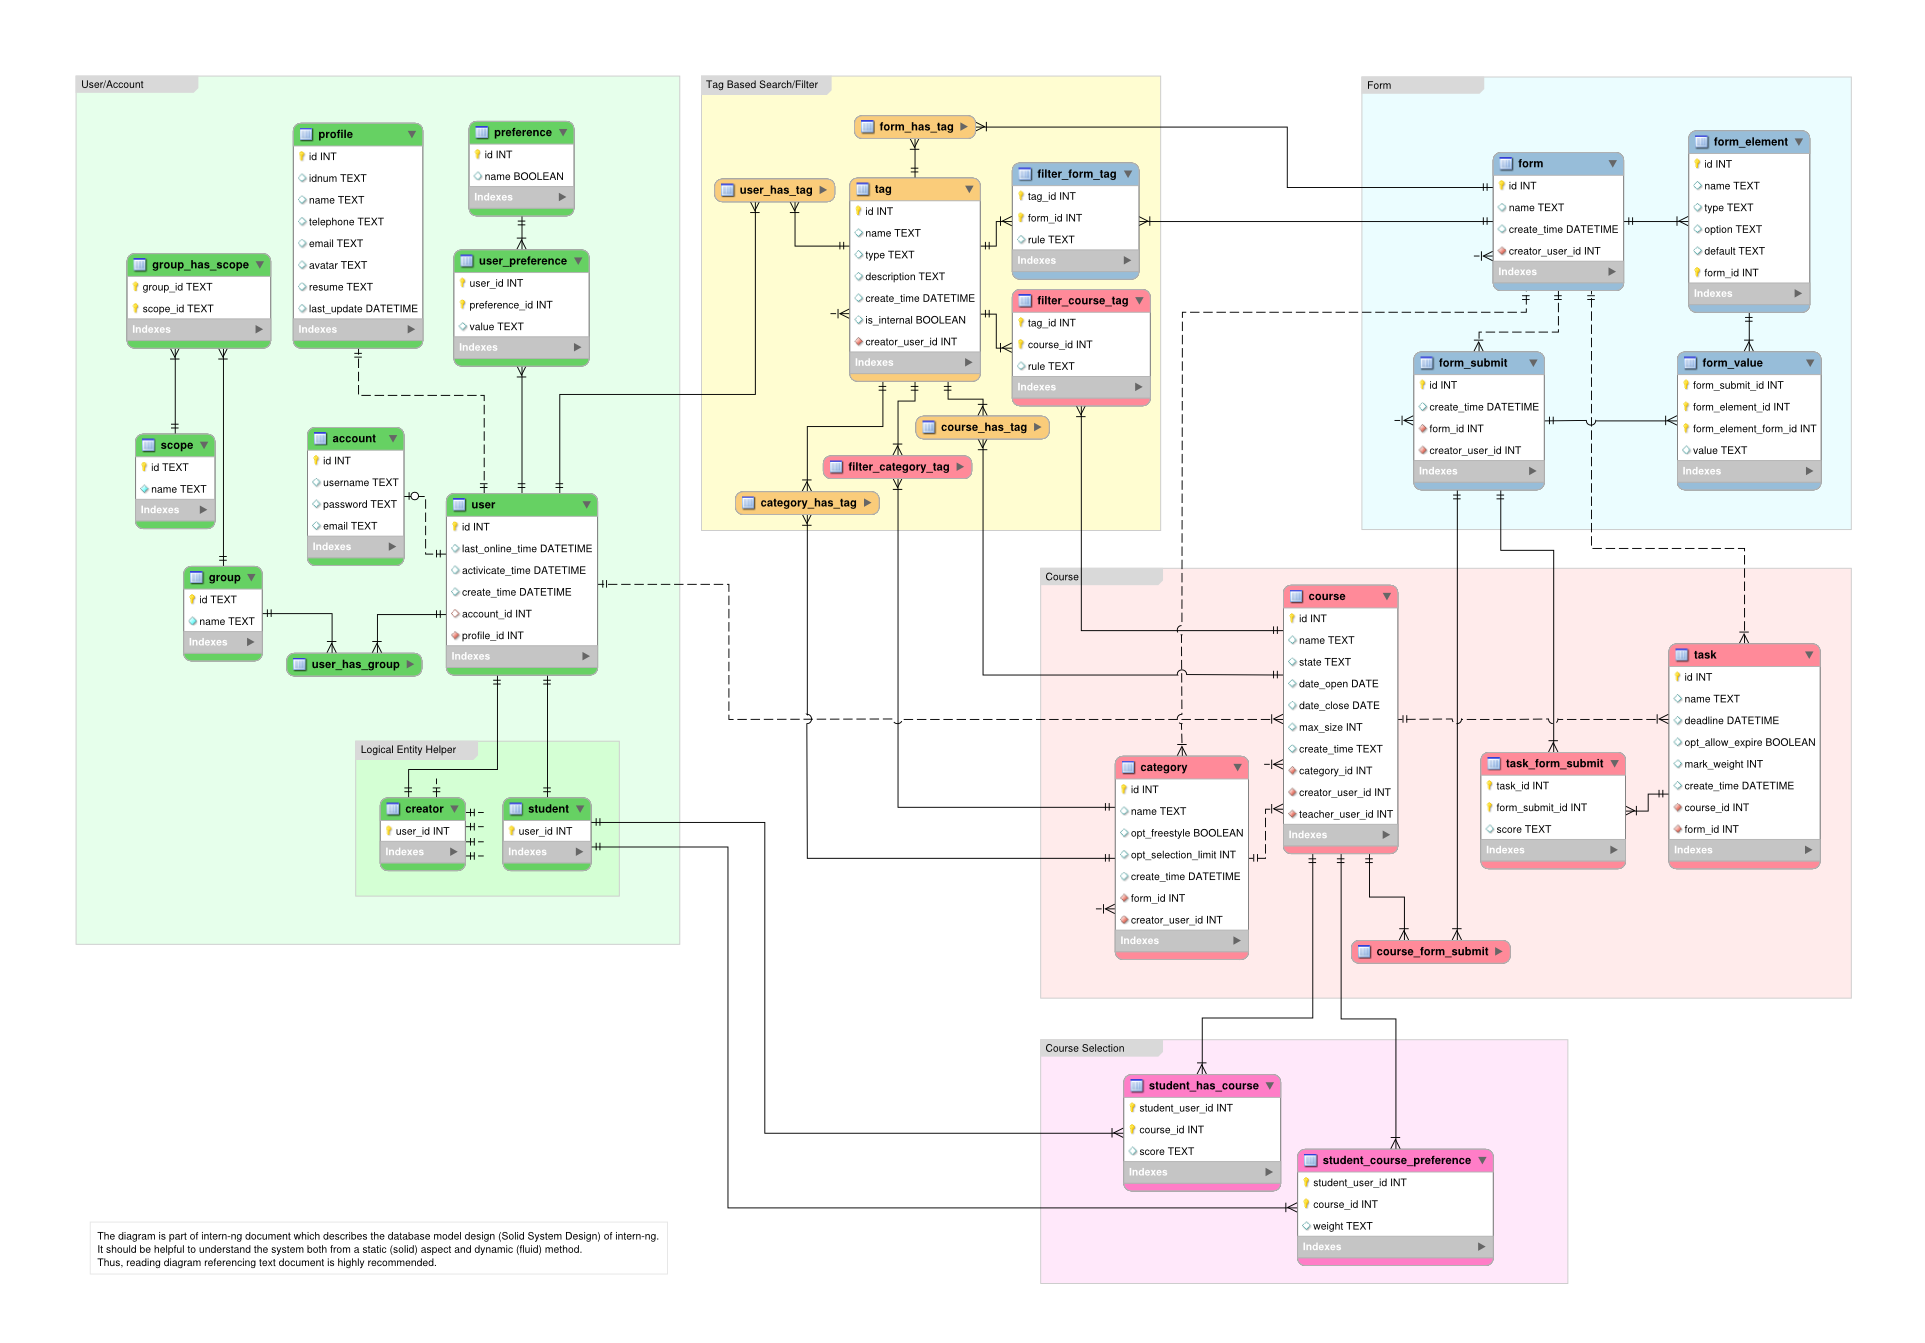
\includegraphics[angle=90, scale=0.5]{figures/eer-120dpi.png} \\
    数据库设计视图\label{FullDatabaseDesign}
  \end{center}
\end{figure}

\newpage

\section*{附录~4\quad	QueryBuilder 模块实现}

\verbatiminput{parts/code/querybuilder.js}

\newpage

\section*{附录~5\quad	Entangle 核心实现}

\verbatiminput{parts/code/entangle.js}

